\documentclass{cursuspresentatie}


\begin{document}
%\input{bib/bib-ref_cmds.tex}
%\input{bib/bib-printbibliography}

\begin{frame}{Bibliografie}
    We gaan de volgende onderwerpen langs
    \begin{itemize}[label=\textbullet]
        \item introductie
        \item bibfile
        \item citeren 
        \item referentielijst
    \end{itemize}
\end{frame}


\begin{saveblock}{codeboxC}
	\begin{minted}{tex}
		\usepackage{biblatex}
		\addbibresource{blablabla.bib}
	\end{minted}
\end{saveblock}

\begin{frame}{Bibliografie}
\begin{itemize}[label=\textbullet]
    \item Je bewaart de gegevens van je bronnen in een apparte bibfile, bijvoorbeeld blablabla.bib
    \item In de preamble roep je dit bibfile aan
    \useblock{codeboxC}
    \item Vervolgens kan je met \mintinline{tex}|\cite{bron}| naar je bibliografie citeren
    \item Let op: je moet zelf de refererentielijst in je document zetten met \mintinline{tex}|\printbibliografy|
\end{itemize}

\end{frame}



\begin{saveblock}{codebox}
	\begin{minted}{bib}
		% File: bibfile.bib
		@article {...
			...
		}
	
		@book {...
			...
		}
		...
	\end{minted}
\end{saveblock}

\begin{saveblock}{codeboxB}
	\begin{minted}{tex}
		% File: document.tex
		\documentclass[a4paper]{article}
		\usepackage{biblatex}
		\addbibresource{bibfile.bib}
		
		\begin{document}
			This has been shown.
			\cite{babington}

			\printbibliography
		\end{document}
	\end{minted}
\end{saveblock}

\begin{frame}{Introductie-voorbeeld}
	% Je hebt dus twee bestanden, die er minimaal zo uitzien.
	% (voor biblatex met backend biber)
	
	\bigskip\medskip
	\begin{columns}
		\begin{column}{0.4\textwidth}
			\useblock{codebox}
		\end{column}%
		\begin{column}{0.6\textwidth}
			\useblock{codeboxB}
		\end{column}
	\end{columns}
\end{frame}



%\input{bib/bib-structure-bibtex}
%willen we natbib noemen? Nee


\begin{saveblock}{codebox}
	\begin{minted}{bib}
		@book{babington,
			author = {Peter Babington},
			title = {Some work},
			publisher = {Publisher},
			year = 1993,
			volume = 4,
			series = 10,
			address = {The address},
			edition = 3,
			month = 7,
			note = {An optional note},
			isbn = {3257227892}
		}
	\end{minted}
\end{saveblock}

\begin{saveblock}{codeboxB}
	\begin{minted}{bib}
		@article{adams,
			author  = {Peter Adams and Hugh Adamsson},
			title   = {Title},
			journal = {Journal},
			year    = 1993,
			number  = 2,
			pages   = {201-213},
			month   = 7,
			note    = {My note}, 
			volume  = 4
		}
	\end{minted}
\end{saveblock}




\begin{saveblock}{codeboxD}
	\begin{minted}{bib}
		@article{adams,
			author  = "Peter Adams and Hugh Adamsson",
			title   = "Title",
			journal = "Journal",
			year    = 1993,
			number  = 2,
			pages   = "201-213",
			month   = 7,
			note    = "My note", 
			volume  = 4
		}
	\end{minted}
\end{saveblock}


\begin{saveblock}{codeboxE}
	\begin{minted}{bib}
		@book{babington,
			author = {Peter Babington},
			title = {Some work},
			publisher = {Publisher},
			year = 1993,
			volume = 4,
			series = 10,
			address = {The address},
			edition = 3,
			month = 7,
			note = {An optional note},
			isbn = {3257227892}
		}
	\end{minted}
\end{saveblock}

\begin{frame}{Bibfile-voorbeeld}
	\useblock{codebox}
\end{frame}

\begin{frame}{Bibfile-voorbeeld}
	\useblock{codeboxB}
\end{frame}


\begin{frame}{Bibfile-voorbeeld}
	\useblock{codeboxD}
\end{frame}


\begin{frame}{Bibfile-voorbeeld}
	\textbf{Niet te vergeten!}
	\begin{itemize}[label=\textbullet]
		\item het eerste argument is waar je naar verwijst \mintinline{tex}|\cite{adams}|\pause
		\item scheid de argumenten met \textbf{komma's!!!}
	\end{itemize}
	\useblock{codeboxB}
\end{frame}
%laat zien hoe het bibliografie bestand in mekaar zit

\updatehighlight{
	name=accentB,
	add={@article}
}

\begin{saveblock}{codeboxa}%
	\begin{minted}{bib}
		@article{Einstein1905,
			author = {A. Einstein},
			title = {\"Uber die von der
				molekularkinetischen Theorie der W\"arme
				geforderte Bewegung von in ruhenden
				Fl\"ussigkeiten suspendierten Teilchen},
			journal = {Annalen der Physik},
			year = 1905,
			volume = 322,
			number = 8,
			pages = {549-560}
		}
	\end{minted}
\end{saveblock}

\begin{frame}{Bibfile-speciale tekens}
	%Hoe ziet een bib-bestand eruit?
	%\begin{center}
	\huge{dit gaat fout!}
	%\bigskip
	\useblock{codeboxa}\medskip
	
	%\LaTeX{} in citaties: gebruik \textcolor{red}{"{} "{}} én \textcolor{red}{ \{ \} }
	%\end{center}
\end{frame}

\begin{saveblock}{codebox}%
	\begin{minted}{bib}
		@article{Einstein1905,
			author = "A. Einstein",
			title = "{\"U}ber die von der
				molekularkinetischen Theorie der W{\"a}rme
				geforderte Bewegung von in ruhenden
				Fl{\"u}ssigkeiten suspendierten Teilchen",
			journal = "Annalen der Physik",
			year = "1905",
			volume = "322",
			number = "8",
			pages = "549-560"
		}
	\end{minted}
\end{saveblock}


\begin{frame}{Bibfile-speciale tekens}
	%Hoe ziet een bib-bestand eruit?
	%\begin{center}
	\huge{Doe het als volgt}
	%\bigskip
	\useblock{codebox}\medskip
	
	%\LaTeX{} in citaties: gebruik \textcolor{red}{"{} "{}} én \textcolor{red}{ \{ \} }
	%\end{center}
\end{frame}

%extra feitjes over de bibliografie 

\begin{frame}{Bibfile-bronvermelding overnemen}
    \centering
    De \texttt{.bib} code hoef je bijna nooit zelf te schrijven!

    \bigskip
    \raggedright
    \begin{itemize}[label=\textbullet]
        \item Op meeste wetenschappelijke websites voor artikels en boeken heb je
    een `export citation' functie. Kies hierbij voor type BibTeX.

        \item Of gebruik een citation manager of browser extension die je hiermee
    helpt. 
    \item chatgpt weet hier ook wel raad mee
    \end{itemize}
    
    % Finding bib code from article sites
\end{frame}


\begin{saveblock}{codebox}%
	\begin{minted}{bib}
		author = {A. Smith and B. Doe and E. Dropper and F. Laker}
	\end{minted}
\end{saveblock}



\begin{frame}{Bibfile-meerdere auteurs}
	
	In je \mintinline{tex}|.bib|-bestand, scheid auteurs met \mintinline{tex}|and|:
	\useblock{codebox}
	Zo kan \mintinline{tex}|biblatex| controleren hoeveel auteurs het toont.\\ \pause
	Dit is belangrijk voor het command \mintinline{tex}|\textcite{source}|:
	\begin{itemize}[label=\textbullet]
		\item \mintinline{tex}|\usepackage{biblatex}| geeft Smith et all \pause
		\item \mintinline{tex}|\usepackage[maxcitenames=5]{biblatex}| geeft Smith, Doe, Dropper and Laker \pause
		\item \mintinline{tex}|\usepackage[maxcitenames=3, mincitenames=2]{biblatex}| geeft Smith, Doe et all \pause
	\end{itemize}
	maxbibnames en minbibnames doen hetzelfde voor je literatuurlijst


	%Voorbeeld: Peter Adams et al.	
\end{frame}

\begin{saveblock}{codebox}%
	\begin{minted}{bib}
		@article{Smith1994,
			author = {A. Smith and B. Doe and E. Dropper},
			title = {Titel},
			journal = {Opt. Lett.},
			year = 1994,
			volume = 19,
			number = 11,
			pages = {780-782}
		}
	\end{minted}
\end{saveblock}


\begin{saveblock}{codeboxB}%
	\begin{minted}{bib}
		@article{Smith1994,
			author = {A. Smith and B. Doe and E. Dropper},
			title = {Titel},
			journal = {Opt. Lett.},
			year = 1994,
			volume = 19,
			number = 11,
			pages = {780-782}
		}
	\end{minted}
\end{saveblock}


%willen we al deze informatie vertellen, dan ga ik het beter uitleggen


\begin{frame}{Citeren-stijl}
	% Bij bibliografie\"en is er een wildernis aan verschillende stijlen:
	Verschillende stijlen zijn mogelijk, onder meer:
	
	\begin{itemize}
		\item \mintinline{tex}|numeric|: This is well-known [2], but also controversial [5, 6].\par
		%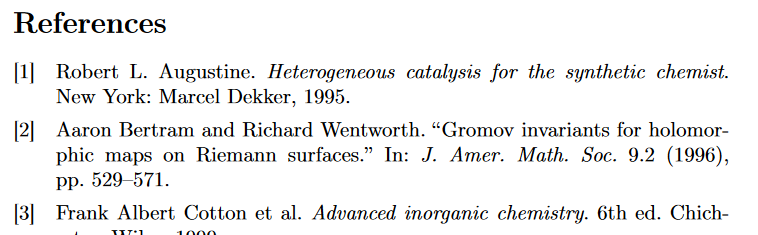
\includegraphics[width=0.8\textwidth]{bib/assets/biblatexStyles/numericReferences.png}
		
		\item \mintinline{tex}|alphabetic|: This is well-known [GMS94], but also controversial [Gon01, Ham97].
		\item \mintinline{tex}|authoryear|: This is well-known John 2003, ...
		\item \mintinline{tex}|apa|: This is well-known (Lambert, 1993), bb ...
	\end{itemize}
	In APA: \mintinline{tex}|\cite| en \mintinline{tex}|\parencite| verschillen
\end{frame}

\begin{saveblock}{codebox}
	%\highlightC{style=numeric}%
	\begin{minted}{tex}
		\usepackage[style=numeric]{biblatex}
	\end{minted}
\end{saveblock}


\begin{saveblock}{codeboxD}%
	\begin{minted}{tex}
		\DeclareLanguageMapping{english}{english-apa}
	\end{minted}
\end{saveblock}

\begin{frame}{Citeren-stijl}
	%En er zijn nog veel meer stijlen!
	Voor exacte wetenschappen: gebruik numeric. Zo
	verander je de stijl:
	\useblock{codebox}
	
	\medskip
	Voor APA-stijl heb je daarnaast nodig:
	\useblock{codeboxD}
	In de preamble van het template staan de verschillende stijlen met uitgebreide uitleg
\end{frame}

%laat de stijlen zien, loop even door de preamble van de template

\newbox\sizetestbox
\savebox\sizetestbox{\mintinline{tex}|\cite{mysource}| en \mintinline{tex}|\parencite{mysource}|}

\newlength\columnfakewidth
\setlength\columnfakewidth{\wd\sizetestbox}
%\setlength\columnfakewidth{\dimexpr\columnfakewidth + 1em\relax}

%\newcommand\firstpart[1]{\atleastwidth[5cm]{#1}}
\newcommand\firstpart[1]{\atleastwidth[\columnfakewidth]{#1}}


\begin{frame}{Citeren-commands}
    In numeric stijl: 
    \begin{itemize}[label=\textbullet]
		\item \firstpart{\mintinline{tex}|\cite{mysource}| en \mintinline{tex}|\parencite{mysource}|}  [1] \pause
		\item \firstpart{\mintinline{tex}|\textcite{mysource}|}  Adams [1] \pause
		\item \firstpart{\mintinline{tex}|\citeauthor{mysource}|}  Adams
		\item \firstpart{\mintinline{tex}|\citeyear{mysource}|}  1991
		\item \firstpart{\mintinline{tex}|\citetitle{mysource}|}  "complex analysis"\pause
		\item \firstpart{\mintinline{tex}|\citeyear{mysource} \cite{mysource}|}  1991 [1]\pause
		\item \firstpart{\mintinline{tex}|\fullcite{mysource}|}  Peter Adams, "..." in: journal enz.
	\end{itemize}
\end{frame}

%\begin{frame}{Citeren-commands}
%    In numeric stijl: 
%    \begin{itemize}[label=\textbullet]
%		\item \firstpart{\mintinline{tex}|\cite{mysource}| en \mintinline{tex}|\parencite{mysource}|}  [1] 
%		\item \firstpart{\mintinline{tex}|\textcite{mysource}|}  Adams [1] 
%		\item \firstpart{\mintinline{tex}|\citeauthor{mysource}|}  Adams
%		\item \firstpart{\mintinline{tex}|\citeyear{mysource}|}  1991
%		\item \firstpart{\mintinline{tex}|\citetitle{mysource}|}  "mathematics is fun"
%		\item \firstpart{\mintinline{tex}|\citeyear{mysource} \cite{mysource}|}  1991 [1]
%		\item \firstpart{\mintinline{tex}|\fullcite{mysource}|}  Peter Adams, "..."\ in: journal enz.
%		\item \firstpart{\mintinline{tex}|\footcite{mysource}|}  tekst\footnote{1}
%	\end{itemize}
%\end{frame}


%\begin{frame}{Citeren-commands}
%    In numeric stijl: 
%    \begin{itemize}[label=\textbullet]
%		\item \firstpart{\mintinline{tex}|\cite{mysource}| en \mintinline{tex}|\parencite{mysource}|}  [1] 
%		\item \firstpart{\mintinline{tex}|\textcite{mysource}|}  Adams [1] 
%		\item \firstpart{\mintinline{tex}|\citeauthor{mysource}|}  Adams
%		\item \firstpart{\mintinline{tex}|\citeyear{mysource}|}  1991
%		\item \firstpart{\mintinline{tex}|\citetitle{mysource}|}  "mathematics is fun"
%		\item \firstpart{\mintinline{tex}|\citeyear{mysource} \cite{mysource}|}  1991 [1]
%		\item \firstpart{\mintinline{tex}|\fullcite{mysource}|}  Peter Adams, "..." in: journal enz.
%		\item \firstpart{\mintinline{tex}|\footcite{mysource}|}  tekst\footnote{1}
%		\item \firstpart{\mintinline{tex}|\footnote{\cite{mysource}}|} tekst\footnote{[1]}
%	\end{itemize}
%\end{frame}
%laat verschillende commando's zijn waarmee je kan citeren


\newbox\sizetestbox
\savebox\sizetestbox{\mintinline{tex}|\cite{mysource}| en \mintinline{tex}|\parencite{mysource}|}


\setlength\columnfakewidth{\wd\sizetestbox}
%\setlength\columnfakewidth{\dimexpr\columnfakewidth + 1em\relax}

%\newcommand\firstpart[1]{\atleastwidth[5cm]{#1}}


\begin{frame}{Citeren-handige trucs}
	Variaties in gebruik:
	
	%	\begin{tabular}{ll}
	%		\lstinline|\\cite\{mysource\}|&[1]\\
	%		\only<2->{\lstinline|\\cite[21]\{mysource\}|&[1, p. 21]\\}
	%		\only<3->{\lstinline|\\cite[21--30,8]\{mysource\}|& [1, pp. 21--30, 8]\\}
	%		\only<4->{\lstinline|\\cite[See][21--30,8]\{mysource\}|& [See 1, pp. 21--30, 8]\\}
	%		\only<5->{\lstinline|\\cite[See chapter 3 of][]\{mysource\}|& [See chapter 3 of 1]\\}
	%		\only<6->{\lstinline|\\cite[See chapter 3 of]\{mysource\}|& [1, See chapter 3 of]\\}
	%		\phantom{\lstinline|\\cite[See chapter 3 of]\{mysource\}|}&\phantom{[1, See chapter 3 of]}
	%	\end{tabular}
	\begin{itemize}[label=\textbullet]
		\item \firstpart{\mintinline{tex}|\cite{mysource}|}  [1] \pause
		\item \firstpart{\mintinline{tex}|\cite[21]{mysource}|}  [1, p. 21] \pause
		\item \firstpart{\mintinline{tex}|\cite[8,21--30]{mysource}|}  [1, pp. 21--30, 8] \pause
		\item \firstpart{\mintinline{tex}|\cite[See][8,21--30]{mysource}|}  [See 1, pp. 21--30, 8] \pause
		\item \firstpart{\mintinline{tex}|\cite[See ch. 3 of][]{mysource}|}  [See ch. 3 of 1] \pause
		\item \firstpart{\mintinline{tex}|\cite[See ch. 3 of]{mysource}|}  [1, See ch. 3 of]\pause
		\item \firstpart{\mintinline{tex}|\cites{mysource}{othsource}|}  [1, 7]\pause
		\item \firstpart{\mintinline{tex}|\cites[8]{mysource}[see ch. 3 of][]{othsource}|}  [1, pp. 8,  ch. 3 of 7]
	\end{itemize}
	
\end{frame}


%\begin{frame}{Citeren-handige trucs}
%	Variaties in gebruik:
	
	
	%\begin{itemize}[label=\textbullet]
	%	\item \firstpart{\mintinline{tex}|\cite{mysource}|}  [1] 
	%	\item \firstpart{\mintinline{tex}|\cite[21]{mysource}|}  [1, p. 21] 
	%	\item \firstpart{\mintinline{tex}|\cite[21--30,8]{mysource}|}  [1, pp. 21--30, 8]
	%	\item \firstpart{\mintinline{tex}|\cite[See][21--30,8]{mysource}|}  [See 1, pp. 21--30, 8]
	%	\item \firstpart{\mintinline{tex}|\cite[See chapter 3 of][]{mysource}|}  [See chapter 3 of 1]
	%	\item \firstpart{\mintinline{tex}|\cite[See chapter 3 of]{mysource}|}  [1, See chapter 3 of]
	%	\item \firstpart{\mintinline{tex}|\cites{mysource}{othsource}|}  [1, 7]
	%	\item \firstpart{\mintinline{tex}|\cites[8]{mysource}[see ch. 3 of][]{othsource}|}  [1, pp. 8,see ch. 3 of 7]
	%	\item \firstpart{\mintinline{tex}|\footcite[this is ... in][]{mysource}|}  tekst \footnote{this is ... in 1}
	%\end{itemize}
	
%\end{frame}

%laat de verschillende citeerstijlen zien

%\input{bib/bib-backend} %wat is dit? Verplaatst naar opmerkingen

% \begin{frame}
%     BibTeX+natbib instead of Biber+biblatex
% \end{frame}



\begin{frame}{Referentielijst-Sortering}
	\begin{itemize}[label=\textbullet]
		\item \mintinline{tex}|\usepackage[sorting=none,...]{biblatex}|: \\
		In volgorde van verschijning in je document

		\item \mintinline{tex}|\usepackage[sorting=nty,...]{biblatex}| (default):\\
		Naam, dan titel, dan jaar

		\item \mintinline{tex}|\usepackage[sorting=nyvt,...]{biblatex}|:\\
		Naam, dan jaar, dan volume, dan titel

		\item \mintinline{tex}|\usepackage[sorting=ydnt,...]{biblatex}|:\\
		Jaar (\underline{d}escending), dan naam, dan titel

		\item Er zijn er nog meer (zie \mintinline{tex}|biblatex| manual, pagina 47)
		
		\item Dit staat ook samengevat in de preamble van de template
	\end{itemize}
\end{frame}



\begin{saveblock}{codebox}
	\begin{minted}{tex}
		\addcontentsline{toc}{section}{References}
	\end{minted}
\end{saveblock}

\begin{frame}{Referentielijst-opmerkingen}%Goed om te weten I}
	\begin{itemize}[label=\textbullet]
		\item Referentielijst is, net zoals \mintinline{tex}|\tableofcontents|, niet standaard opgenomen in je
		inhoudstabel. Dit fix je met
		\useblock{codebox}\pause
		
		\item Enkel citaties die je hebt gebruikt verschijnen in je \mintinline{tex}|\printbibliography|.
		\item Mocht je toch alle citaties uit je \mintinline{tex}|.bib|-bestand in referentielijst willen:\\
		Gebruik \mintinline{tex}|\nocite{*}|, met * de bron waar je nog niet naar hebt verwezen \pause
		\item Zet standaard aan \mintinline{tex}|\usepackage[backend=biber]{biblatex}|
	\end{itemize}
\end{frame}

% \begin{frame}{Goed om te weten II}
% 	\hll|biber| verzorgt een groot deel van de refentielijst, maar wordt niet bij elke compilatie
% 	aangeroepen. Het wordt aangeroepen als	
% 	\begin{itemize}
% 		\item De hulpbestanden (.aux, .bbl, ...) nog genoeg missen.
% 		\item Je in TeXstudio gebruikt \hll|Tools > Bibliography| (F8).
% 		\item Je een nieuwe bron gebruikt in je \hll|.tex|-bestand.
% 		\item TeXstudio ziet dat \hll|.bib|-bestand aangepast is.
% 	\end{itemize}

% 	Maar dus \emph{niet} gewoon omdat je de een paragraaf verwijdert die de laatste citatie van een
% 	referentie had. Doe je zoiets op het laatste moment voor inleveren, compileer, F8, en compileer
% 	nogmaals.
% \end{frame}


\end{document}